\documentclass{beamer}

\usepackage{listings}
\usepackage[color]{circus}
\usepackage{tikz}
\usepackage{amsthm}
\usepackage{algorithmicx}
\usepackage{algpseudocode}
\usepackage{algorithm}
\usepackage[loadonly]{enumitem}

\lstset{language=C}

\usetikzlibrary{calc}

\tikzset{onslide/.code args={<#1>#2}{\only<#1>{\pgfkeysalso{#2}}}}

\newtheorem{rul}{Rule}

\usetheme[compress]{Dresden}
% \setbeamertemplate{navigation symbols}{}
\setbeamertemplate{footline}{
  \leavevmode%
  \hbox{%
  \begin{beamercolorbox}[wd=.25\paperwidth,ht=2.25ex,dp=1ex,center]{author in head/foot}%
    \usebeamerfont{author in head/foot}\insertshortauthor
  \end{beamercolorbox}%
  \begin{beamercolorbox}[wd=.5\paperwidth,ht=2.25ex,dp=1ex,center]{title in head/foot}%
    \usebeamerfont{title in head/foot}\insertshorttitle
  \end{beamercolorbox}%
  \begin{beamercolorbox}[wd=.25\paperwidth,ht=2.25ex,dp=1ex,right]{date in head/foot}%
    \usebeamerfont{date in head/foot}\insertshortdate{}\hspace*{2em}
    \insertframenumber{} \hspace*{2ex}
  \end{beamercolorbox}}%
  \vskip0pt%
} 
\usecolortheme{rose}

\renewlist{itemize}{itemize}{4}
\setlist[itemize]{label=\usebeamerfont*{itemize item}%
  \usebeamercolor[fg]{itemize item}
  \usebeamertemplate{itemize item},
  leftmargin=1cm,
  labelindent=\parindent,
  itemsep=1pt}
\setlist[itemize,1]{leftmargin=0.3cm}
\setlist[itemize,2]{before*=\small}

% \renewcommand{\insertsectionnumber}{}
% \renewcommand{\sectionname}{}


\title[An Approach to Verification of Ahead-of-time Compilation for
  SCJ]{An Approach to Verification of\\Ahead-of-time Compilation for\\
  Safety-Critical Java}
\author{James Baxter}
\date[2018-03-20]{Thesis Seminar\\20 March 2018}

\begin{document}

\frame[plain]{\titlepage}

\begin{frame}
\frametitle{Outline}
\tableofcontents
\end{frame}

\section{Introduction}
\stepcounter{subsection}

\begin{frame}
  \frametitle{Motivation}
  \begin{itemize}
  \item Java for real-time and embedded systems
  \item Safety-Critical Java (SCJ)
  \item Differences from standard Java
    \begin{itemize}
    \item Scheduling
    \item Memory management
    \item No dynamic class loading
    \end{itemize}
  \item Requires a specialised SCJ virtual machine (SCJVM)
  \item Existing SCJVMs:~icecap HVM, Fiji VM, OVM
    \begin{itemize}
    \item Compilation for efficiency
    \item No formal verification
    \item icecap:~the only publicly-available up-to-date SCJVM
    \end{itemize}
  \end{itemize}
\end{frame}

\begin{frame}
  \frametitle{Compiler Correctness}
  \begin{itemize}
  \item Our aim: verification of compilation from SCJ bytecode to C
    \begin{itemize}
    \item following the approach of icecap
    \end{itemize}
  \item Two main approaches to compiler verification:
    \begin{itemize}
    \item commuting diagram approach
    \item algebraic approach 
    \end{itemize}
  \end{itemize}
\end{frame}

\begin{frame}
  \frametitle{Commuting diagram approach}
  \begin{itemize}
  \item Define functions for source and target semantics
  \item Also define an \emph{encode function}, which maps source meanings to target meanings
  \item Compilation is correct if this diagram commutes:
  \end{itemize}
  \begin{center}
    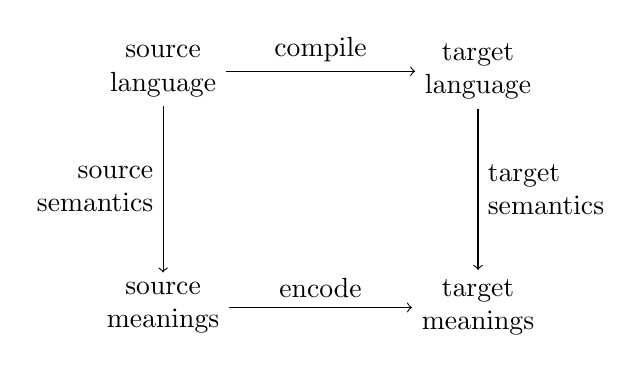
\begin{tikzpicture}
      \node[align=center] (S) at (0cm,3cm) {source\\language};
      \node[align=center] (T) at (4cm,3cm) {target\\language};
      \node[align=center] (M) at (0cm,0cm) {source\\meanings};
      \node[align=center] (U) at (4cm,0cm) {target\\meanings};
      
      \path (S) edge[->] node[align=center, above] {compile}           (T);
      \path (S) edge[->] node[align=right, left]   {source\\semantics} (M);
      \path (T) edge[->] node[align=left, right]   {target\\semantics} (U);
      \path (M) edge[->] node[align=center, above] {encode}            (U);
    \end{tikzpicture}
  \end{center}
\end{frame}

\begin{frame}
  \frametitle{Algebraic Approach}
  \begin{itemize}
  \item Define source and target in same specification language
  \item Correct compilation is described by \emph{refinement}
  \end{itemize}
  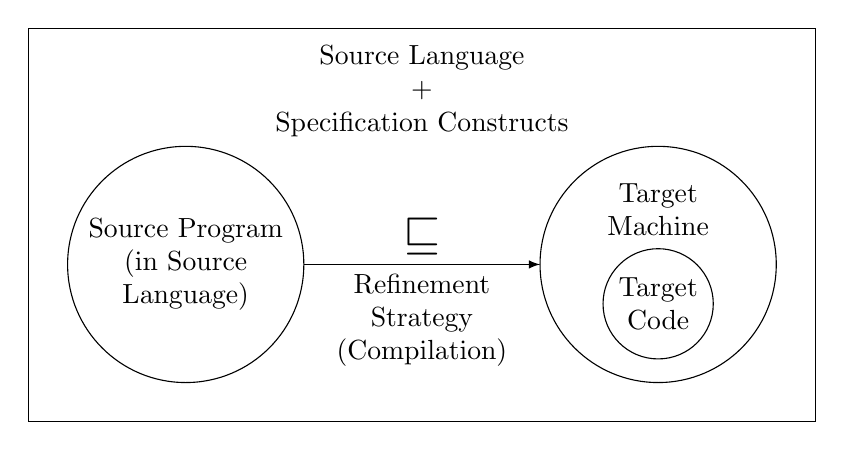
\begin{tikzpicture}
    \draw (0cm,0cm) |- (10cm,5cm) |- (0cm,0cm);
    \draw (5cm,4.2cm) node[align=center] {Source Language\\+\\Specification Constructs};

    \draw (2cm,2cm)   circle[radius=1.5cm]               node[align=center] {Source Program\\(in Source\\Language)};
    \draw (8cm,2cm)   circle[radius=1.5cm] ++(0cm,0.7cm) node[align=center] {Target\\Machine};
    \draw (8cm,1.5cm) circle[radius=0.7]                 node[align=center] {Target\\Code};

    \path (3.5cm,2cm) edge[-latex] 
              node[align=center, above] {\LARGE $\sqsubseteq$} 
              node[align=center, below] {Refinement\\Strategy\\(Compilation)}  
          (6.5cm,2cm);
  \end{tikzpicture}
\end{frame}

% Remember to say why this approach is taken
\begin{frame}
  \frametitle{Our Approach}
  \begin{itemize}
  \item Reverse of standard algebraic approach
  \item Java bytecode semantics is defined in terms of its VM
  \item C code defined by shallow embedding in the specification language
  \end{itemize}
  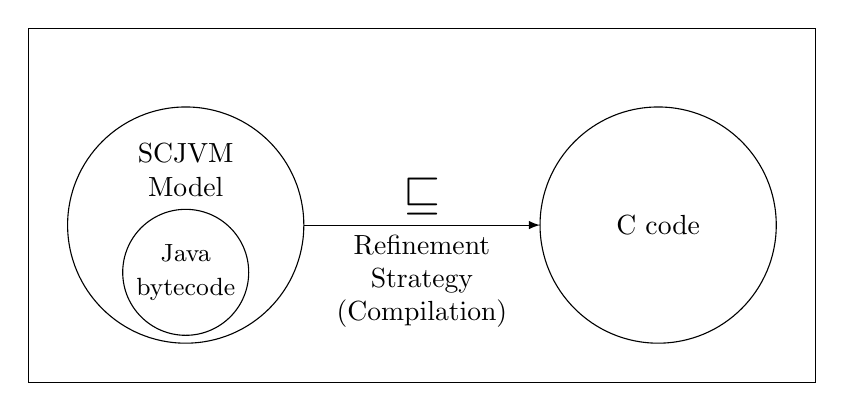
\begin{tikzpicture}
    \draw (0cm,0cm) rectangle (10cm,4.5cm);
    \draw (5cm,4.2cm) node[align=center] {\Circus{}};

    \draw (8cm,2cm)   circle[radius=1.5cm]               node[align=center] {C code};
    \draw (2cm,2cm)   circle[radius=1.5cm] ++(0cm,0.7cm) node[align=center] {SCJVM\\Model};
    \draw (2cm,1.4cm) circle[radius=0.8]                 node[align=center] {\small Java \\\small bytecode};

    \path (3.5cm,2cm) edge[-latex] 
              node[align=center, above] {\LARGE $\sqsubseteq$} 
              node[align=center, below] {Refinement\\Strategy\\(Compilation)}  
          (6.5cm,2cm);
  \end{tikzpicture}
\end{frame}

\begin{frame}[shrink,squeeze]
  \frametitle{\Circus{}}
  \scriptsize
  \begin{itemize}
  \item Based on CSP and the Z notation
  \item CSP to specify processes that communicate over channels
  \item Z to specify state and data operations
  \item Processes have encapsulated state and may be made up of
    multiple actions.
  \item Channels represent the interface of a process.
  \item Processes may be composed in parallel.
  \item Notation for refinement
  \end{itemize}
  %\vspace{-0.5cm}
  \begin{columns}[T]
    \tiny
    \setlength{\zedindent}{0cm}
    \setlength{\zedleftsep}{0.1cm}
    \setlength{\zedtab}{0.5cm}
    \setlength{\abovedisplayskip}{0cm}
    \setlength{\abovedisplayshortskip}{0cm}
    \setlength{\belowdisplayskip}{0cm}
    \setlength{\belowdisplayshortskip}{0cm}
    \column{0.5\textwidth}
  \begin{circus}
    \circchannel getInstruction : ProgramAddress \\
    \circchannel getInstructionRet : Bytecode \\
  \end{circus}
  \vspace{-0.6cm}
  \begin{circus}
    \t2 \vdots
  \end{circus}
  \begin{circus}
    \circprocess Interpreter \circdef \circbegin
  \end{circus}
  \begin{schema}{InterpreterState}
    frameStack : \seq StackFrame \\
    pc : ProgramAddress \\
    currentClass : Class
  \where
    % definition of currentClass (only important if the frame stack is nonempty)
  frameStack \neq \emptyset \implies \\
  \t1 currentClass = \\
  \t2 (last~frameStack).frameClass
  \end{schema}
  \begin{circusaction}
    \circstate InterpreterState
  \end{circusaction}
  \vfill
  \column{0.5\textwidth}
  \begin{schema}{InterpreterInit}
    InterpreterState~'
  \where
    frameStack' = \emptyset
  \end{schema}
  \vspace{-0.4cm}
  \begin{circusaction}
    \t2\vdots
  \end{circusaction}
  \begin{circusaction}
    Loop \circdef \\
    \t1 \left(\begin{array}{l}
          \lcircguard frameStack \neq \emptyset \rcircguard \circguard HandleInstruction \\
          {} \extchoice {} \\
          \lcircguard frameStack = \emptyset \rcircguard \circguard StartInterpreter
        \end{array}\right) \circseq \\
    \t1 Loop
  \end{circusaction}
  \begin{circusaction}
    \circspot \lschexpract InterpreterInit \rschexpract \circseq Loop
  \end{circusaction}
  \begin{circus}
    \circend
  \end{circus}
  \vfill
\end{columns}
\end{frame}

\begin{frame}
  \frametitle{Contributions}
  \begin{itemize}
  \item Formal model of an interpreting SCJVM
  \item Compilation strategy
    \begin{itemize}
    \item Acts on Java bytecode in the interpreter
    \item Outputs a shallow embedding of C code
    \item Specification of how to apply compilation rules
    \end{itemize}
  \item Compilation rules
    \begin{itemize}
    \item Formal rules, with proofs of correctness
    \item Stated using refinement
    \item Act on the interpreter model
    \end{itemize}
  \end{itemize}
\end{frame}

\begin{frame}
  \frametitle{Safety-Critical Java}
  \begin{itemize}
  \item An SCJ program is made up of missions, which are executed sequentially, in an order determined by a \texttt{MissionSequencer}.
  \item A class implementing the \texttt{Safelet} interface initialises the program and supplies the \texttt{MissionSequencer}.
  \item Each mission is made up of event handlers of various types:
    \begin{itemize}
      \item aperiodic handlers, which execute in response to release
        requests;
      \item periodic handlers, which execute repeatedly at set
        time periods;
      \item one-shot handlers, which execute once after a set time period.
      \end{itemize}
  % \item Memory is allocated in memory areas with different lifetimes.
  % \item Annotations allow for checking that dangling references cannot occur.
  \end{itemize}
  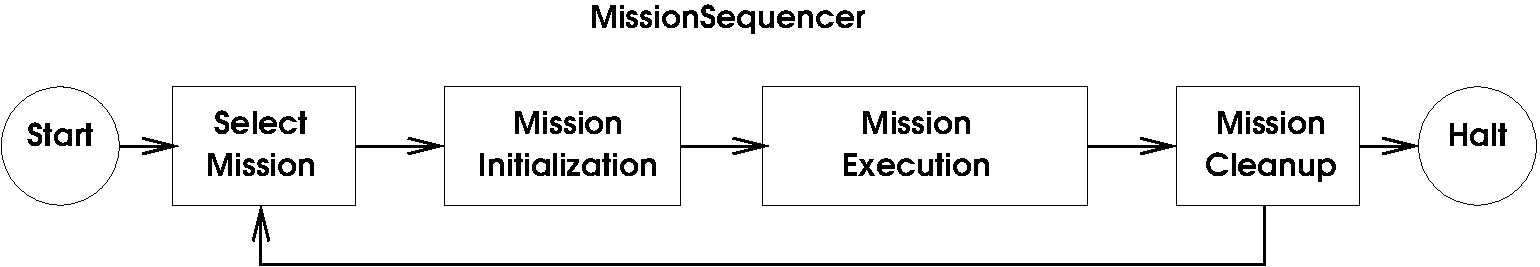
\includegraphics[width=\textwidth]{phases.pdf}
\end{frame}

\begin{frame}
  \frametitle{Safety-Critical Java}
  \begin{columns}
    \begin{column}{.5\textwidth}
      \begin{itemize}
      \item Memory is allocated in memory areas with different lifetimes:
        \begin{itemize}
        \item immortal memory
        \item mission memory
        \item per-release memory
        \item temporary private memory
        \end{itemize}
      \item Annotations allow for checking that dangling references cannot occur.
      \end{itemize}
    \end{column}
    \begin{column}{.5\textwidth}
      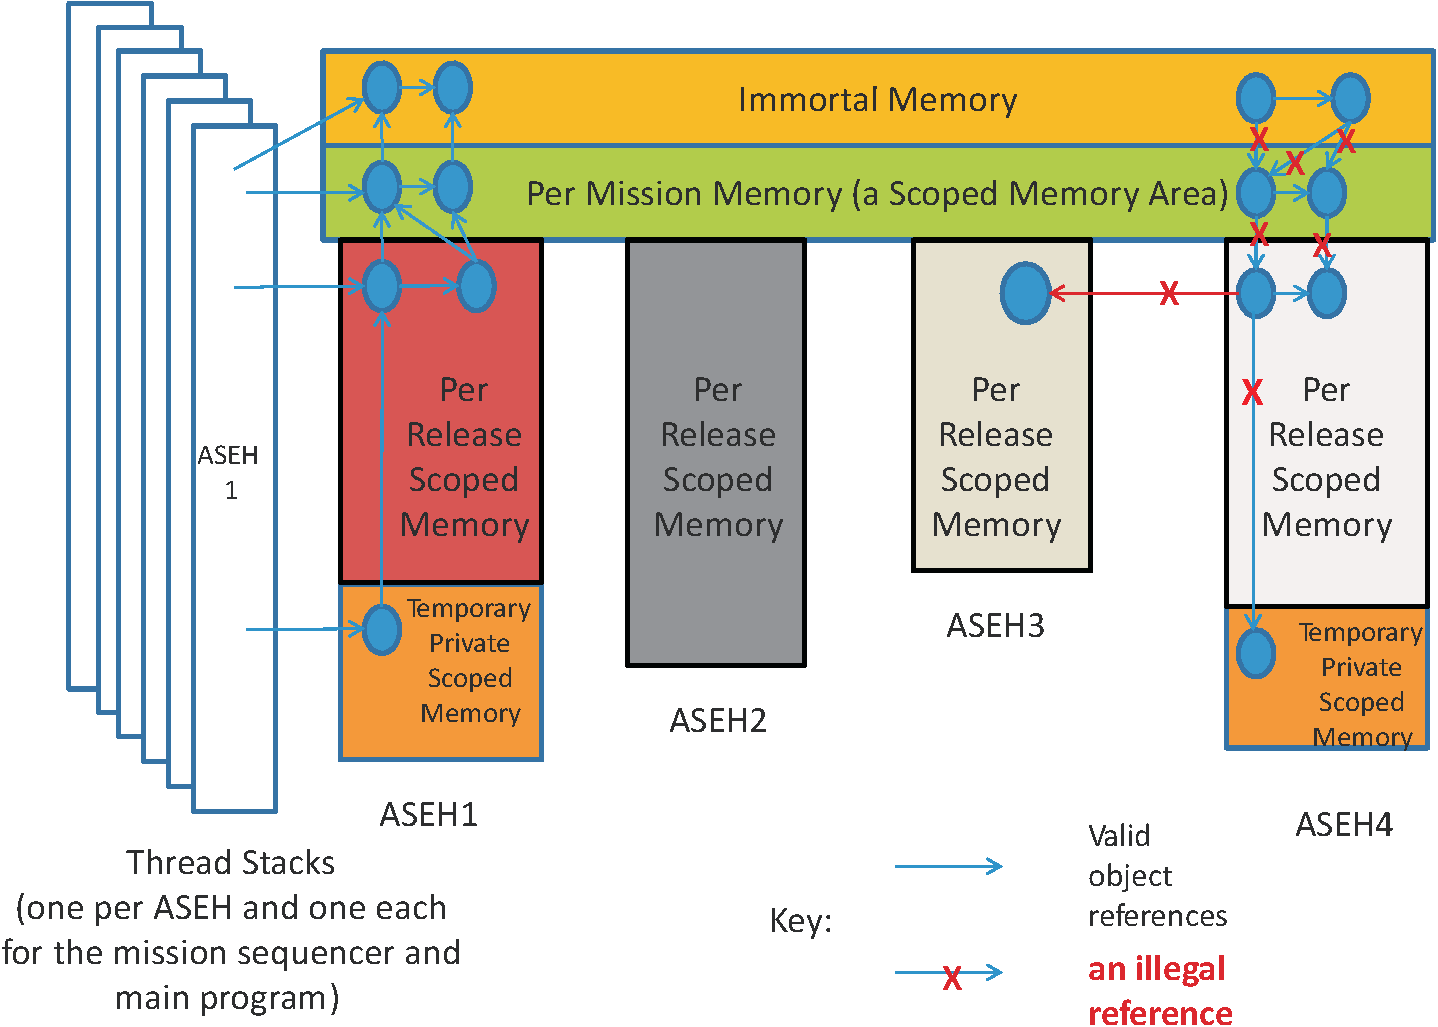
\includegraphics[width=\textwidth]{Stacks-Areas.pdf}
    \end{column}
  \end{columns}
\end{frame}
  
\section{SCJVM Model}
\stepcounter{subsection}

\begin{frame}
  \frametitle{Overview of Model}
  \centering
  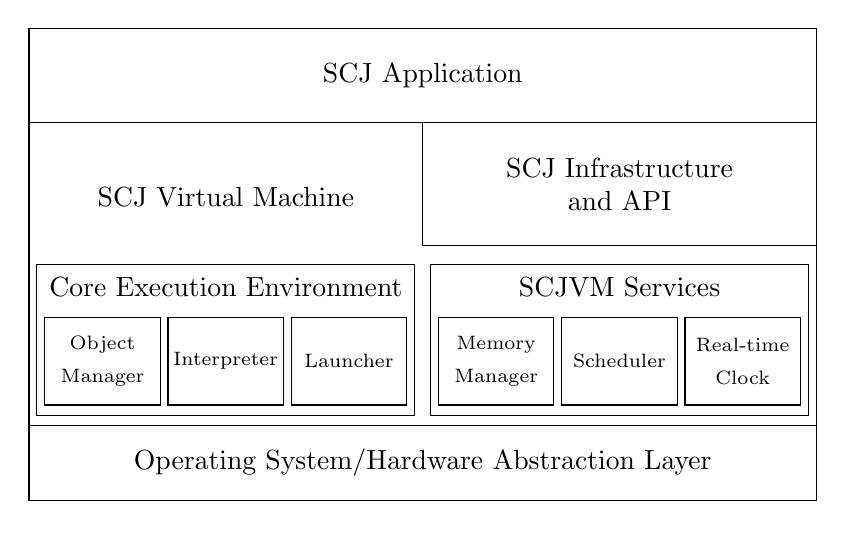
\begin{tikzpicture}
    \coordinate (width)  at (10cm,0cm);
    \coordinate (height) at (0cm,6cm);

    \path (0,0) -- (height)
    coordinate[pos=0.16] (OS boundary)
    coordinate[pos=0.18] (VM part bottom)
    coordinate[pos=0.50] (VM part top)
    coordinate[pos=0.54] (API boundary)
    coordinate[pos=0.80] (App boundary);

    \path (VM part bottom) -- (VM part top)
    coordinate[pos=0.65] (VM Service top)
    coordinate[pos=0.65] (CEE part top);

    \path (VM part bottom) -- (VM part top)
    coordinate[pos=0.85] (CEE ypos)
    coordinate[pos=0.85] (VM Services ypos);

    \path (0,0) -- (width)
    coordinate[pos=0.01] (CEE left)
    coordinate[pos=0.49] (CEE right)
    coordinate[pos=0.51] (VM Services left)
    coordinate[pos=0.99] (VM Services right)
    coordinate[pos=0.01] (CEE part sep)
    coordinate[pos=0.01] (VM Service sep);

    \path (CEE left) -- (CEE right)
    coordinate[pos=0.5] (CEE xpos);

    \path (VM Services left) -- (VM Services right)
    coordinate[pos=0.5] (VM Services xpos);

    \path (0,0) to node[pos=0.5] (mid) {} (width);
    \path (0,0) to node[pos=0.25] (quart) {} (width);

    \draw (0,0) rectangle (width |- height);

    \draw (OS boundary) -- ++(width);
    \path (0,0) rectangle node[pos=0.5] (OS) {} (width |- OS boundary);
    \draw (mid |- API boundary) rectangle node[pos=0.5] (API) {} (width |- App boundary);
    \draw (App boundary) -- ++(width);
    \path (App boundary) rectangle node[pos=0.5] (App) {} (width |- height);

    \path (quart |- API boundary) rectangle node[pos=0.4] (SCJVM) {} (quart |- App boundary);
    \draw[onslide=<2->{color=red}] (VM Services left |- VM part bottom) rectangle (VM Services right |- VM part top);
    \draw[onslide=<2->{color=red}] (CEE left |- VM part bottom) rectangle (CEE right |- VM part top);
    \coordinate (CEE) at (CEE xpos |- CEE ypos);
    \coordinate (VM Services) at (VM Services xpos |- VM Services ypos);

    \node[align=center] at (App)   {SCJ Application};
    \node[align=center] at (API)   {SCJ Infrastructure\\and API};
    \node[align=center, onslide=<2->{color=red}] at (SCJVM) {SCJ Virtual Machine};
    \node[align=center, onslide=<2->{color=red}] at (CEE)   {Core Execution Environment};
    \node[align=center, onslide=<2->{color=red}] at (VM Services)  {SCJVM Services};
    \node[align=center] at (OS)    {Operating System/Hardware Abstraction Layer};

    \foreach \x in {1,...,3}
    \pgfmathsetmacro{\a}{0.333*(\x - 1)}
    \pgfmathsetmacro{\b}{0.333*\x}
    \path ($(CEE left) + (VM part bottom)!0.07!(VM part top)$) --
    node[pos=\a] (CEE part \x start) {}
    node[pos=\b] (CEE part \x end) {}
    ($(CEE right) + (VM part bottom)!0.07!(VM part top) - (CEE part sep)$);

    \foreach \x in {1,...,3}
    \draw[onslide=<2->{color=red}] ($(CEE part \x start) + (CEE part sep)$)
    rectangle node[pos=0.5] (CEE part \x) {}
    (CEE part \x end |- CEE part top);

    \node[align=center, onslide=<2->{color=red}] at (CEE part 1) {\scriptsize Object \\ \scriptsize Manager};
    \node[align=center, onslide=<2->{color=red}] at (CEE part 2) {\scriptsize Interpreter};
    \node[align=center, onslide=<2->{color=red}] at (CEE part 3) {\scriptsize Launcher};

    \foreach \x in {1,...,3}
    \pgfmathsetmacro{\a}{0.333*(\x - 1)}
    \pgfmathsetmacro{\b}{0.333*\x}
    \path ($(VM Services left) + (VM part bottom)!0.07!(VM part top)$) --
    node[pos=\a] (VM Service \x start) {}
    node[pos=\b] (VM Service \x end) {}
    ($(VM Services right) + (VM part bottom)!0.07!(VM part top) - (VM Service sep)$);

    \foreach \x in {1,...,3}
    \draw[onslide=<2->{color=red}] ($(VM Service \x start) + (VM Service sep)$)
    rectangle node[pos=0.5] (VM Service \x) {}
    (VM Service \x end |- VM Service top);

    \node[align=center, onslide=<2->{color=red}] at (VM Service 1) {\scriptsize Memory \\ \scriptsize Manager};
    \node[align=center, onslide=<2->{color=red}] at (VM Service 2) {\scriptsize Scheduler};
    \node[align=center, onslide=<2->{color=red}] at (VM Service 3) {\scriptsize Real-time \\ \scriptsize Clock};
  \end{tikzpicture}
\end{frame}

\subsection{SCJVM Services}
%\stepcounter{subsection}

\begin{frame}
  \frametitle{Memory Manager}
  \begin{itemize}
  \item Deals with \emph{backing stores} --- low level blocks of
    memory that underlie memory areas
  \item The \emph{root
      backing store} covers the whole of backing store memory.
  \item Backing stores may have backing stores nested within them.
  \item Operations on backing stores:~clearing, resizing, allocating
    memory and backing stores, locating the backing store of an object
    % \begin{itemize}
    % \item obtaining information on a backing store: total size, free size etc.\
    % \item allocating one backing store within another
    % \item allocating memory for an object in a backing store
    % \item locating the backing store of a particular object
    % \item clearing a backing store
    % \item resizing a backing store
    % \end{itemize}
  \item The Memory Manager also deals with allocating stacks, which
    are stored in a separate area from backing stores.
  \end{itemize}
\end{frame}

\begin{frame}
  \frametitle{Scheduler}
  \begin{itemize}
  \item The SCJVM schedules \emph{threads} --- abstract lines of
  execution used to implement SCJ's event handlers.
  % \item Threads transition between different states.
  \item Threads eligible to execute are scheduled using priority queues.
    \begin{itemize}
    \item The thread at the front of the highest-priority queue is $current$.
    \end{itemize}
  \item Locking on objects using priority-ceiling emulation.
  \item Interrupts are scheduled as if they were threads.
  \end{itemize}
  
  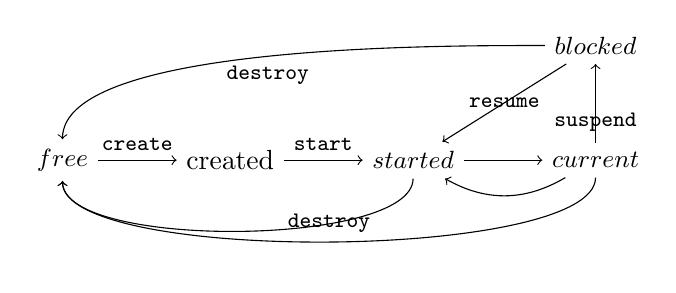
\begin{tikzpicture}
    \usetikzlibrary{positioning}
    \node (free)    at (0,0)        {\small $free$};
    \node (created) [right=of free] {created};
    \node (started) [right=of created] {\small $started$};
    \node (current) [right=of started] {\small $current$};
    \node (blocked) [above=of current] {\small $blocked$};
    
    \draw[->] (free)    edge node[above] {\footnotesize \texttt{create}} (created);
    \draw[->] (created) edge node[above] {\footnotesize \texttt{start}} (started);
    \draw[->] (current) edge node[below] {\footnotesize \texttt{suspend}} (blocked);
    \draw[->] (blocked) edge node {\footnotesize \texttt{resume}} (started);
    \draw[->] (started) edge             (current);
    \draw[->] (current) edge[bend left]  (started);

    \draw[->] (current) edge[looseness=0.4, out=270, in=270] node[above] {\footnotesize \texttt{destroy}} (free);
    \draw[->] (started) edge[looseness=0.5, out=270, in=270] (free);
    \draw[->] (blocked) edge[looseness=0.5, out=180, in=90]  node[below] {\footnotesize \texttt{destroy}} (free);
  \end{tikzpicture}
\end{frame}

\begin{frame}
  \frametitle{Real-time Clock}
  \begin{itemize}
  \item Supplies the current time, as a millisecond-nanosecond pair
  \item Time kept via clock tick interrupts from hardware
  \item Allows an alarm to be set to send an interrupt at a specific time
  \end{itemize}
\end{frame}

\subsection{CEE Model}
%\stepcounter{subsection}

\begin{frame}
  \frametitle{Overview of CEE model}
  \begin{itemize}
  \item Core Execution Environment (CEE) has three components:
    \begin{itemize}
    \item Launcher
    \item Object Manager
      % \begin{itemize}
      % \item manages object representation and memory areas
      % \end{itemize}
    \item Interpreter 
      % \begin{itemize}
      % \item handles execution of individual bytecodes
      % \end{itemize}
    
      % \begin{itemize}
      % \item manages SCJVM startup and coordinates mission execution
      % \end{itemize}
    \end{itemize}
  \item CEE parameters:
    \begin{itemize}
    \item Bytecode instructions ($bc$)
    \item Classes ($cs$)
    \item \texttt{Safelet} identifier ($sid$)
    \item Class initialisation order ($initOrder$)
    \end{itemize}
  \end{itemize}
  \vspace{-0.8cm}
  {\setlength{\zedindent}{2mm}
    \setlength{\zedleftsep}{2mm}
    \setlength{\zedtab}{0.7em}
    \begin{circus}
      \circprocess CEE(bc,cs,sid,initOrder) \circdef \\
      \t1 ObjMan(cs) \parallel Interpreter(bc,cs)  \parallel Launcher(sid,initOrder)
    \end{circus}}
\end{frame}

\begin{frame}
  \frametitle{Launcher}
  \begin{itemize}
  \item Manages SCJVM startup and coordinates mission execution
  \item Operates by instructing the Interpreter to execute methods
  \item Models part of the SCJ infrastructure
  \item Unaffected by compilation strategy
  \end{itemize}
\end{frame}

\begin{frame}
  \frametitle{Object Manager}
  \begin{itemize}
  \item Manages the representation of objects
  \item Each object is stored as a structure containing its class
    information and a map from field identifiers to values.
  \item Also tracks the current backing store in use by each thread
    \begin{itemize}
    \item Used to allocate space when creating a new object
    \end{itemize}
  \end{itemize}
\end{frame}

\begin{frame}
  \frametitle{Interpreter}
  \begin{itemize}
  \item Each thread is represented by a separate \Circus{} process.
  \item The state of each thread's process contains the program counter
    and frame stack.
  \item {The Interpreter is a parallel composition of these threads.
      \setlength{\zedindent}{0cm}
      \setlength{\zedleftsep}{0cm}
      \setlength{\abovedisplayskip}{0.1cm}
      \setlength{\belowdisplayskip}{0.1cm}
      \begin{circus}
        \circprocess Interpreter(bc,cs) \circdef \Parallel t : TID \setminus \{ idle \} \circspot Thr(bc, cs, t)
      \end{circus}}
  \item The thread processes proceed through a sequence of different
    actions as the scheduler starts and switches between them.
  \end{itemize}
  \centering
  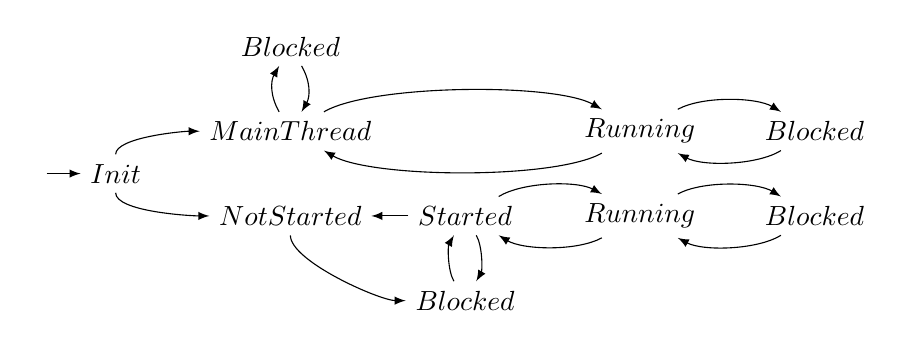
\begin{tikzpicture}
    \node at (9cm,0) (width) {};
    \node at (0,1.2cm) (height) {};

    \path (0,0) --
    node[pos=0.00] (Initxpos) {}
    node[pos=0.25] (MainThreadxpos) {}
    node[pos=0.25] (NotStartedxpos) {}
    node[pos=0.50] (Startedxpos) {}
    node[pos=0.75] (Runningxpos) {}
    node[pos=1.00] (Blockedxpos) {}
    (width);

    \path (0,0) --
    node[pos=-1]  (threadBlockedypos) {}
    node[pos=0]   (threadypos) {}
    node[pos=0.5] (Initypos) {}
    node[pos=1]   (mainypos) {}
    node[pos=2]   (mainBlockedypos) {}
    (height);

    \path (Initxpos |- Initypos) node (Init) {$Init$} ++(-1cm,0cm) node (start) {};
    \node at (MainThreadxpos |- mainypos) (IMn) {$MainThread$};
    \node at (Runningxpos |- mainypos) (MRn) {$Running$};
    \node at (MainThreadxpos |- mainBlockedypos) (MBl) {$Blocked$};
    \node at (Blockedxpos |- mainypos) (MB2) {$Blocked$};
    \node at (NotStartedxpos |- threadypos) (NSt) {$NotStarted$};
    \node at (Startedxpos |- threadypos) (Sta) {$Started$};
    \node at (Startedxpos |- threadBlockedypos) (TBl) {$Blocked$};
    \node at (Runningxpos |- threadypos) (TRn) {$Running$};
    \node at (Blockedxpos |- threadypos) (TB2) {$Blocked$};

    \draw[-latex] (start) to (Init);
    \draw[-latex] (Init) to[out=90,in=180,looseness=0.5] (IMn);
    \draw[-latex] (Init) to[out=270,in=180,looseness=0.5] (NSt);
    \draw[-latex] (IMn) to[bend left,looseness=0.5] (MRn);
    \draw[-latex] (MRn) to[bend left,looseness=0.5] (IMn);
    \draw[-latex] (MRn) to[bend left,looseness=0.7] (MB2);
    \draw[-latex] (MB2) to[bend left,looseness=0.7] (MRn);
    \draw[-latex] (IMn) to[bend left,looseness=1.0] (MBl);
    \draw[-latex] (MBl) to[bend left,looseness=1.0] (IMn);
    \draw[-latex] (NSt) to[out=270,in=180,looseness=0.5] (TBl);
    \draw[-latex] (TBl) to[bend left,looseness=0.7] (Sta);
    \draw[-latex] (Sta) to[bend left,looseness=0.7] (TBl);
    \draw[-latex] (Sta) to (NSt);
    \draw[-latex] (Sta) to[bend left,looseness=0.7] (TRn);
    \draw[-latex] (TRn) to[bend left,looseness=0.7] (Sta);
    \draw[-latex] (TB2) to[bend left,looseness=0.7] (TRn);
    \draw[-latex] (TRn) to[bend left,looseness=0.7] (TB2);
  \end{tikzpicture}
\end{frame}

\begin{frame}
  \frametitle{C Code Representation}
  \begin{itemize}
  \item {\setlength{\zedindent}{0cm}
      \setlength{\zedleftsep}{0cm}
      \setlength{\abovedisplayskip}{0.1cm}
      \setlength{\belowdisplayskip}{0.1cm}
      \setlength{\abovedisplayshortskip}{0.1cm}
      \setlength{\belowdisplayshortskip}{0.1cm}
      The C code is represented by processes representing C threads.
      \begin{circus}
        \circprocess CProg_{bc,cs} \circdef \Parallel t : ThreadID \setminus \{ idle \} \circspot CThr_{bc,cs}(t)
      \end{circus}}
  \item Each function is a separate action in the process.
  \item Function arguments are represented by action parameters.
  \item C variables are represented by \Circus{} variable blocks.
  \item \Circus{} recursion and conditionals represent C loops and conditionals.
  \item Objects are structs represented by Z schema bindings.
  \end{itemize}
\end{frame}

\section{Compilation Strategy}
\stepcounter{subsection}

% \begin{frame}
%   \frametitle{Overview of Compilation Strategy}
%   \begin{tikzpicture}
%     \draw (0cm,0.4cm) rectangle (10cm,4.5cm);
%     \draw (5cm,4.2cm) node[align=center] {\scriptsize Specification Language (\Circus{})};

%     \draw (2cm,2.8cm)   circle[radius=1.5cm] ++(0cm,0.6cm) node[align=center] {\scriptsize Core\\\scriptsize Execution\\\scriptsize Environment};
%     \draw (2cm,1.95cm)     circle[radius=0.6cm]               node[align=center] {\scriptsize Bytecode};
%     \draw (8cm,2.8cm)   circle[radius=1.5cm]               node[align=center] {\scriptsize C Code};

%     \draw (1cm,0.5cm) rectangle (3cm,1.3cm) node[pos=0.5,align=center] {\scriptsize SCJVM \\\scriptsize Services};
%     \draw (7cm,0.5cm) rectangle (9cm,1.3cm) node[pos=0.5,align=center] {\scriptsize SCJVM \\\scriptsize Services};

%     \path (3.5cm,2.8cm) edge[-latex]
%     node[align=center, above] {\Large $\sqsubseteq$}
%     node[align=center, below] {\scriptsize Refinement\\\scriptsize Strategy\\\scriptsize (Compilation)}
%     (6.5cm,2.8cm);

%     % \draw[-latex] (3cm,0.9cm) -- (7cm,0.9cm);
%   \end{tikzpicture}
% \end{frame}

\begin{frame}
  \frametitle{Overview of Compilation Strategy}
  \begin{itemize}
  \item Applies compilation rules to transform the interpreter.
  \item Divided into three stages:
    \begin{itemize}
    \item Elimination of Program Counter
    \item Elimination of Frame Stack
    \item Data Refinement of Memory
    \end{itemize}
  \end{itemize}
\end{frame}

\begin{frame}[fragile,shrink]
  \frametitle{Example Program}
\begin{lstlisting}[language=Java]
public class InputHandler extends PeriodicEventHandler {
    
  private InputStream input;
  private Buffer buffer;
  
  public InputHandler(PriorityParameters priority,
                      PeriodicParameters release,
                      StorageParameters storage,
                      ConfigurationParameters config,
                      InputStream input, Buffer buffer) {
    super(priority, release, storage, config);
	
    this.input = input;
    this.buffer = buffer;
  }

  public void handleAsyncEvent() {
    try {
      int value = input.read();
      buffer.put(value);
    } catch (IOException e) {
    }
  }
  
}
\end{lstlisting}
\end{frame}

\begin{frame}
  \frametitle{Example Program}
  \tiny
  \setlength{\zedleftsep}{0cm}
  \setlength{\zedindent}{0cm}
  \setlength{\zedtab}{0.3cm}
  \setlength{\abovedisplayskip}{0cm}
  \setlength{\abovedisplayshortskip}{0cm}
  \setlength{\belowdisplayskip}{0cm}
  \setlength{\belowdisplayshortskip}{0cm}
  \begin{columns}[T]
    \column{.3\textwidth}
    \begin{axdef}
      bc : ProgramAddress \pfun Bytecode
    \where
      programMemory = \{ \\
      \t1 0 \mapsto aload~0, \\
      \t1 1 \mapsto aload~1, \\
      \t1 2 \mapsto aload~2, \\
      \t1 3 \mapsto aload~3, \\
      \t1 4 \mapsto aload~4, \\
      \t1 5 \mapsto invokespecial~12, \\
      \t1 6 \mapsto aload~0, \\
      \t1 7 \mapsto aload~5, \\
      \t1 8 \mapsto putfield~15, \\
      \t1 9 \mapsto aload~0, \\
      \t1 10 \mapsto aload~6, \\
      \t1 11 \mapsto putfield~17, \\
      \t1 12 \mapsto return, \\
      \t1 13 \mapsto aload~0, \\
      \t1 14 \mapsto getfield~15, \\
      \t1 15 \mapsto invokevirtual~33, \\
      \t1 16 \mapsto astore~1, \\
      \t1 17 \mapsto aload~0, \\
      \t1 18 \mapsto getfield~17, \\
      \t1 19 \mapsto aload~1, \\
      \t1 20 \mapsto invokevirtual~39, \\
      \t1 21 \mapsto goto~2, \\
      \t1 22 \mapsto astore~1, \\
      \t1 23 \mapsto return \\
      \t1 \dots \\
      \} 
    \end{axdef}
    \column{.7\textwidth}
    \begin{axdef}
      InputHandler : Class
    \where
      InputHandler = \lblot \\
      \t1 constantPool == \{ \\
      \t2 1 \mapsto ClassRef~InputHandlerID, \\
      \t2 3 \mapsto ClassRef~PeriodicEventHandlerID, \\
      \t2 12 \mapsto MethodRef~(PeriodicEventHandlerID, PEHinit), \\
      \t2 15 \mapsto FieldRef~(InputHandlerID,input), \\
      \t2 17 \mapsto FieldRef~(InputHandlerID,buffer), \\
      \t2 33 \mapsto MethodRef(InputStreamID,read), \\
      \t2 34 \mapsto ClassRef~InputStreamID, \\
      \t2 39 \mapsto MethodRef~(BufferID,put), \\
      \t2 40 \mapsto ClassRef~BufferID \\
      \t1 \}, \\
      \t1 this == 1, \\
      \t1 super == 3, \\
      \t1 interfaces == \{\}, \\
      \t1 methodEntry == \{ init \mapsto 0, handleAsyncEvent \mapsto 13 \}, \\
      \t1 methodEnd == \{ init \mapsto 12, handleAsyncEvent \mapsto 23 \}, \\
      \t1 methodLocals == \{ init \mapsto 7, handleAsyncEvent \mapsto 2 \}, \\
      \t1 methodStackSize == \{ init \mapsto 5, handleAsyncEvent \mapsto 2 \}, \\
      \t1 fields == \{ input, buffer \}, \\
      \t1 staticFields == \{\} \\
      \rblot
    \end{axdef}
    
    \begin{axdef}
      cs : ClassID \pfun Class
    \where
      cs = \{ InputHandlerID \mapsto InputHandler, \dots \}
    \end{axdef}
  \end{columns}
\end{frame}

\subsection{Elimination of Program Counter}

\begin{frame}
  \frametitle{Elimination of Program Counter}
  \begin{itemize}
  \item Operates on the $Thr$ processes of the interpreter
  \item Introduces the control flow constructs of the C code.
  \item Copies methods into separate actions.
  \item Removes program counter from state.
  \end{itemize}
\end{frame}

\begin{frame}
  \frametitle{Elimination of Program Counter}
  \begin{algorithm}[H]
    \begin{algorithmic}[1]
      \State \Call{ExpandBytecode}{}
      \State \Call{IntroduceSequentialComposition}{}
      \While{$\lnot$\Call{AllMethodsSeparated}{}}
      \State \Call{IntroduceLoopsAndConditionals}{}
      \State \Call{SeparateCompleteMethods}{}
      \State \Call{ResolveMethodCalls}{}
      \EndWhile
      \State \Call{RefineMainActions}{}
      \State \Call{RemovePCFromState}{}
    \end{algorithmic}
    \caption{Elimination of Program Counter}
  \end{algorithm}
\end{frame}

\begin{frame}
  \frametitle{Elimination of Program Counter}
  \centering
  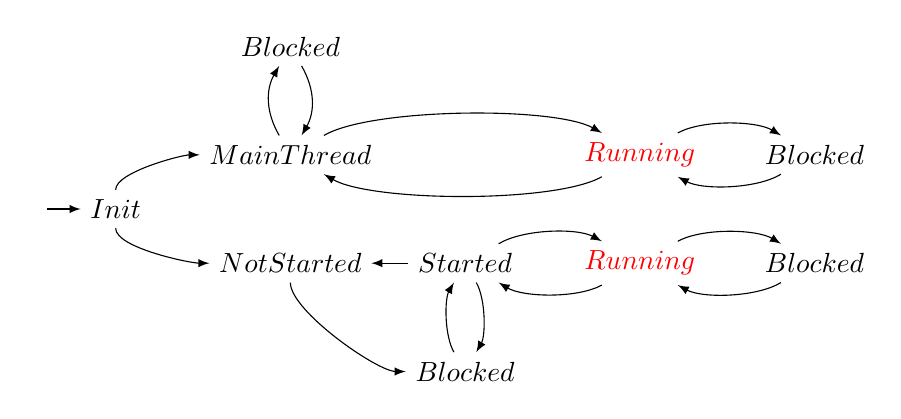
\begin{tikzpicture}
    \node at (9cm,0) (width) {};
    \node at (0,1.5cm) (height) {};

    \path (0,0) --
    node[pos=0.00] (Initxpos) {}
    node[pos=0.25] (MainThreadxpos) {}
    node[pos=0.25] (NotStartedxpos) {}
    node[pos=0.50] (Startedxpos) {}
    node[pos=0.75] (Runningxpos) {}
    node[pos=1.00] (Blockedxpos) {}
    (width);

    \path (0,0) --
    node[pos=-1]  (threadBlockedypos) {}
    node[pos=0]   (threadypos) {}
    node[pos=0.5] (Initypos) {}
    node[pos=1]   (mainypos) {}
    node[pos=2]   (mainBlockedypos) {}
    (height);

    \path (Initxpos |- Initypos) node (Init) {$Init$} ++(-1cm,0cm) node (start) {};
    \node at (MainThreadxpos |- mainypos) (IMn) {$MainThread$};
    \node at (Runningxpos |- mainypos) (MRn) {\color{red} $Running$};
    \node at (MainThreadxpos |- mainBlockedypos) (MBl) {$Blocked$};
    \node at (Blockedxpos |- mainypos) (MB2) {$Blocked$};
    \node at (NotStartedxpos |- threadypos) (NSt) {$NotStarted$};
    \node at (Startedxpos |- threadypos) (Sta) {$Started$};
    \node at (Startedxpos |- threadBlockedypos) (TBl) {$Blocked$};
    \node at (Runningxpos |- threadypos) (TRn) {\color{red} $Running$};
    \node at (Blockedxpos |- threadypos) (TB2) {$Blocked$};

    \draw[-latex] (start) to (Init);
    \draw[-latex] (Init) to[out=90,in=180,looseness=0.5] (IMn);
    \draw[-latex] (Init) to[out=270,in=180,looseness=0.5] (NSt);
    \draw[-latex] (IMn) to[bend left,looseness=0.5] (MRn);
    \draw[-latex] (MRn) to[bend left,looseness=0.5] (IMn);
    \draw[-latex] (MRn) to[bend left,looseness=0.7] (MB2);
    \draw[-latex] (MB2) to[bend left,looseness=0.7] (MRn);
    \draw[-latex] (IMn) to[bend left,looseness=1.0] (MBl);
    \draw[-latex] (MBl) to[bend left,looseness=1.0] (IMn);
    \draw[-latex] (NSt) to[out=270,in=180,looseness=0.5] (TBl);
    \draw[-latex] (TBl) to[bend left,looseness=0.7] (Sta);
    \draw[-latex] (Sta) to[bend left,looseness=0.7] (TBl);
    \draw[-latex] (Sta) to (NSt);
    \draw[-latex] (Sta) to[bend left,looseness=0.7] (TRn);
    \draw[-latex] (TRn) to[bend left,looseness=0.7] (Sta);
    \draw[-latex] (TB2) to[bend left,looseness=0.7] (TRn);
    \draw[-latex] (TRn) to[bend left,looseness=0.7] (TB2);
  \end{tikzpicture}
\end{frame}

\begin{frame}
  \frametitle{Bytecode Expansion}
  \tiny
  \setlength{\abovedisplayskip}{0cm}
  \setlength{\abovedisplayshortskip}{0cm}
  \setlength{\belowdisplayskip}{0cm}
  \setlength{\belowdisplayshortskip}{0cm}
  \vspace{-0.2cm}
  \begin{circus}
    Running \circdef \begin{array}[t]{l}
                       \circif frameStack = \emptyset \circthen \Skip \\
                       {} \circelse frameStack \neq \emptyset \circthen {} \\
                       \t1 {} \circif pc = 0 \circthen HandleAload(0) \circseq pc := 1 \\
                       \t1 {} \circelse pc = 1 \circthen HandleAload(1) \circseq pc := 2 \\
                       \t1 {} \circelse pc = 2 \circthen HandleAload(2) \circseq pc := 3 \\
                       \t1 {} \circelse pc = 3 \circthen HandleAload(3) \circseq pc := 4 \\
                       \t1 {} \circelse pc = 4 \circthen HandleAload(4) \circseq pc := 5 \\
                       \t1 {} \circelse pc = 5 \circthen HandleInvokespecial(12) \\
                       \t1 {} \circelse pc = 6 \circthen HandleAload(0) \circseq pc := 7 \\
                       \t1 {} \circelse pc = 7 \circthen HandleAload(5) \circseq pc := 8 \\
                       \t1 {} \circelse pc = 8 \circthen HandlePutfield(15) \circseq pc := 9 \\
                       \t1 {} \circelse pc = 9 \circthen HandleAload(0) \circseq pc := 10 \\
                       \t1 {} \circelse pc = 10 \circthen HandleAload(6) \circseq pc := 11 \\
                       \t1 {} \circelse pc = 11 \circthen HandlePutfield(17) \circseq pc := 12 \\
                       \t1 {} \circelse pc = 12 \circthen HandleReturn \\
                       \t1 {} \circelse pc = 13 \circthen HandleAload(0) \circseq pc := 14 \\
                       \t1 {} \circelse pc = 14 \circthen HandleGetfield(15) \circseq pc := 15 \\
                       \t1 {} \circelse pc = 15 \circthen HandleInvokevirtual(33) \\
                       \t1 {} \circelse pc = 16 \circthen HandleAstore(1) \circseq pc := 17 \\
                       \t1 {} \circelse pc = 17 \circthen HandleAload(0) \circseq pc := 18 \\
                       \t1 {} \circelse pc = 18 \circthen HandleGetfield(17) \circseq pc := 19 \\
                       \t1 {} \circelse pc = 19 \circthen HandleAload(1) \circseq pc := 20 \\
                       \t1 {} \circelse pc = 20 \circthen HandleInvokevirtual(39) \\
                       \t1 {} \circelse pc = 21 \circthen pc := 23 \\
                       \t1 {} \circelse pc = 22 \circthen HandleAstore(1) \circseq pc := 23 \\
                       \t1 {} \circelse pc = 23 \circthen HandleReturn \\
                       \t1 \dots \\
                       \t1 {} \circfi \circseq Poll \circseq Running \\
                       \circfi
                     \end{array}
  \end{circus}
\end{frame}

\begin{frame}
  \frametitle{Compilation Rules}
  \small
  \begin{rul}[Sequence introduction]
    \label{sequence-introduction-rule}
    \setlength{\zedindent}{0cm}
    \setlength{\zedtab}{0.5cm}
    \setlength{\abovedisplayskip}{0.1cm}
    \setlength{\belowdisplayskip}{0.1cm}
    If $i \neq j$ and
    \begin{circus}
      \{frameStack \neq \emptyset\} \circseq A {} \;\; = \;\; 
      \{frameStack \neq \emptyset\} \circseq A \circseq \{frameStack \neq \emptyset\}
    \end{circus}
    then,
    \begin{circus}
      \begin{array}{l}
        \circmu X \circspot \\
        \t1  \circif frameStack = \emptyset \circthen \Skip \\
        \t1  {} \circelse frameStack \neq \emptyset \circthen {} \\
        \t2 \circif {} \cdots {} \\
        \t2 {} \circelse pc = i \circthen \\
        \t3 A \circseq pc := j \\
        \t2 {} \circelse pc = j \circthen B \\
        \t2 {} \cdots {} \\
        \t2 \circfi \circseq Poll \circseq X \\
        \t1 \circfi
      \end{array}
      \circrefines_A
      \begin{array}{l}
        \circmu X \circspot \\
        \t1 \circif frameStack = \emptyset \circthen \Skip \\
        \t1 {} \circelse frameStack \neq \emptyset \circthen {} \\
        \t2 \circif {} \cdots {} \\
        \t2 {} \circelse pc = i \circthen {} \\
        \t3 A \circseq pc := j \circseq Poll \circseq B \\
        \t2 {} \circelse pc = j \circthen B \\
        \t2 {} \cdots {} \\
        \t2 \circfi \circseq Poll \circseq X \\
        \t1 \circfi
      \end{array}
    \end{circus}
  \end{rul}
\end{frame}

\begin{frame}
  \frametitle{Method Separation}
  \centering
  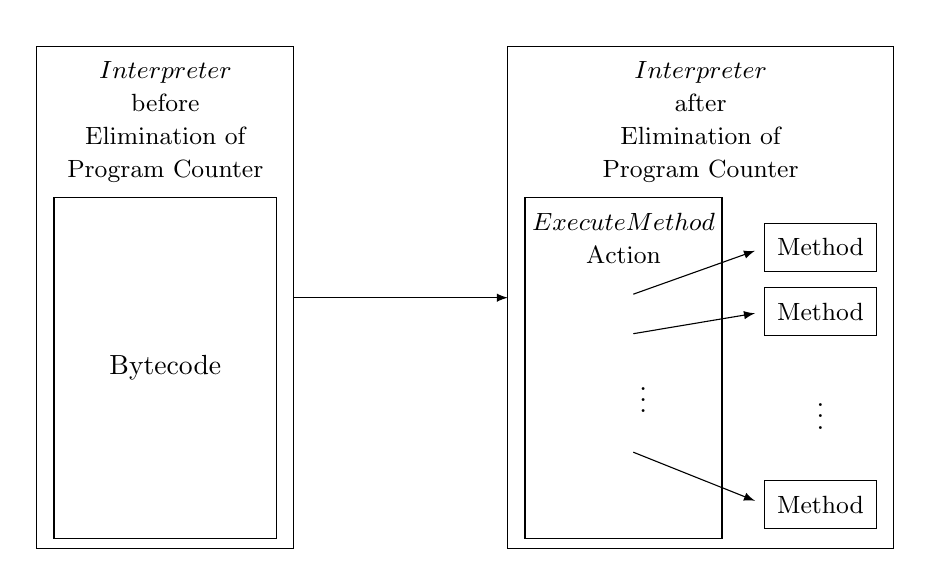
\begin{tikzpicture}
    \node at (11cm,0) (width) {};
    \node at (0,6.5cm) (height) {};

    \path (0,0) --
    node[pos=0.00] (Interpreter1Left) {}
    node[pos=0.02] (BytecodeLeft) {}
    node[pos=0.28] (BytecodeRight) {}
    node[pos=0.30] (Interpreter1Right) {}
    node[pos=0.50] (CenterXPos) {}
    node[pos=0.55] (Interpreter2Left) {}
    node[pos=0.57] (ExecuteMethodLeft) {}
    node[pos=0.685] (ExecuteMethodAnchorsXPos) {}
    node[pos=0.80] (ExecuteMethodRight) {}
    node[pos=0.85] (MethodsLeft) {}
    node[pos=0.98] (MethodsRight) {}
    node[pos=1.00] (Interpreter2Right) {}
    (width);

    \path (0,0) --
    node[pos=0.00] (InterpreterBot) {}
    node[pos=0.02] (ContentsBot) {}
    node[pos=0.20] (ExecuteMethodAnchorsBot) {}
    node[pos=0.50] (CenterYPos) {}
    node[pos=0.50] (ExecuteMethodAnchorsTop) {}
    node[pos=0.70] (ContentsTop) {}
    node[pos=1.00] (InterpreterTop) {}
    (height);

    \draw (Interpreter1Left |- InterpreterBot) rectangle
    (Interpreter1Right |- InterpreterTop);
    \draw (Interpreter2Left |- InterpreterBot) rectangle
    (Interpreter2Right |- InterpreterTop);

    \draw (BytecodeLeft |- ContentsBot) rectangle
    node[pos=0.5,align=center] {Bytecode}
    (BytecodeRight |- ContentsTop);
    \draw (ExecuteMethodLeft |- ContentsBot) rectangle
    (ExecuteMethodRight |- ContentsTop);    
    \path (ExecuteMethodAnchorsXPos |- ContentsBot) --
    node[pos=0.88,align=center] {\small $ExecuteMethod$\\\small Action}
    (ExecuteMethodAnchorsXPos |- ContentsTop);
    
    \path (Interpreter1Left |- ContentsTop) rectangle
    node[pos=0.5,align=center] {\small $Interpreter$\\\small before\\\small Elimination of\\\small Program Counter}
    (Interpreter1Right |- InterpreterTop);
    \path (Interpreter2Left |- ContentsTop) rectangle
    node[pos=0.5,align=center] {\small $Interpreter$\\\small after\\\small Elimination of\\\small Program Counter}
    (Interpreter2Right |- InterpreterTop);
    
    \foreach \x in {1,...,5}
    \pgfmathsetmacro{\a}{0.2*(\x - 1)}
    \pgfmathsetmacro{\b}{0.2*(\x - 1) + 0.15}
    \path (ContentsBot) --
    node[pos=\a] (Method\x Bot) {}
    node[pos=\b] (Method\x Top) {}
    (ContentsTop);

    \foreach \x in {1,...,5}
    \path (MethodsLeft |- Method\x Bot) --
    node[pos=0.5] (Method\x Anchor) {}
    (MethodsLeft |- Method\x Top);

    \foreach \x in {1,...,5}
    \pgfmathsetmacro{\a}{0.25*(\x - 1)}
    \path (ExecuteMethodAnchorsXPos |- ExecuteMethodAnchorsBot) --
    node[pos=\a] (ExecuteMethodAnchor\x ) {}
    (ExecuteMethodAnchorsXPos |- ExecuteMethodAnchorsTop);
    
    \draw (MethodsLeft |- Method1Bot) rectangle
    node[pos=0.5] {\small Method}
    (MethodsRight |- Method1Top);
    \draw (MethodsLeft |- Method4Bot) rectangle
    node[pos=0.5] {\small Method}
    (MethodsRight |- Method4Top);
    \draw (MethodsLeft |- Method5Bot) rectangle
    node[pos=0.5] {\small Method}
    (MethodsRight |- Method5Top);
    \path (MethodsLeft |- Method2Bot) rectangle
    node[pos=0.5,align=center] {\vdots}
    (MethodsRight |- Method3Top);

    \draw[-latex] (ExecuteMethodAnchor1) -- (Method1Anchor);
    \draw[-latex] (ExecuteMethodAnchor4) -- (Method4Anchor);
    \draw[-latex] (ExecuteMethodAnchor5) -- (Method5Anchor);
    \path (ExecuteMethodAnchor2) --
    node[pos=0.5,align=center] {\hspace{0.5cm}\vdots}
    (ExecuteMethodAnchor3);

    \draw[-latex] (Interpreter1Right |- CenterYPos) --
    node[above] {\huge $\circrefines$}
    (Interpreter2Left |- CenterYPos);
  \end{tikzpicture}
\end{frame}

\begin{frame}[shrink]
  \frametitle{Resulting Code}
  \setlength{\zedleftsep}{0cm}
  \setlength{\zedindent}{0cm}
  \begin{circus}
    InputHandler\_init \circdef HandleAload(0) \circseq Poll \circseq HandleAload(1) \circseq \\
    \t1 Poll \circseq HandleAload(2) \circseq Poll \circseq HandleAload(3) \circseq Poll \circseq \\
    \t1 HandleAload(4) \circseq Poll \circseq (\circvar poppedArgs : \seq Word \circspot \\
    \t2 \lschexpract \exists argsToPop? == e @ InterpreterStackFrameInvoke \rschexpract \circseq \\
    \t2 \lschexpract InterpreterNewStackFrame[ \\
    \t3 PeriodicEventHandler/class?,  init/methodID?, poppedArgs/methodArgs?] \rschexpract) \circseq Poll \circseq \\
    \t1 PeriodicEventHandler\_init \circseq Poll \circseq HandleAload(0) \circseq Poll \circseq \\
    \t1 HandleAload(5) \circseq Poll \circseq HandlePutfield(15) \circseq Poll \circseq \\
    \t1 HandleAload(0) \circseq Poll \circseq HandleAload(6) \circseq Poll \circseq \\
    \t1 HandlePutfield(17) \circseq Poll \circseq HandleReturn
  \end{circus}
  \begin{circus}
    InputHandler\_handleAsyncEvent \circdef HandleAload(0) \circseq Poll \circseq \\
    \t1 HandleGetfield(15) \circseq Poll \circseq (\circvar poppedArgs : \seq Word \circspot \\
    \t2 \lschexpract \exists argsToPop? == e @ InterpreterStackFrameInvoke \rschexpract \circseq \\
    \t2 \lschexpract InterpreterNewStackFrame[ \\
    \t3 Inputter/class?,  read/methodID?, poppedArgs/methodArgs?] \rschexpract) \circseq Poll \circseq \\
    \t1 Inputter\_read \circseq Poll \circseq HandleAstore(1) \circseq Poll \circseq \\
    \t1 HandleAload(0) \circseq Poll \circseq HandleGetfield(17) \circseq Poll \circseq \\
    \t1 HandleAload(1) \circseq Poll \circseq (\circvar poppedArgs : \seq Word \circspot \\
      \t2 \lschexpract \exists argsToPop? == e @ InterpreterStackFrameInvoke \rschexpract \circseq \\
      \t2 \lschexpract InterpreterNewStackFrame[ \\
      \t3 Buffer/class?,  put/methodID?, poppedArgs/methodArgs?] \rschexpract) \circseq Poll \circseq \\
    \t1 Buffer\_Put \circseq Poll \circseq Poll \circseq HandleReturn
  \end{circus}
\end{frame}

\subsection{Elimination of Frame Stack}

\begin{frame}
  \frametitle{Elimination of Frame Stack}
  \begin{itemize}
  \item Introduces variables and parameters representing Java local
    variables and operand stack slots.
  \item Removes the frame stack from the state, copying its
    information to the introduced variables.
  \end{itemize}
\end{frame}

\begin{frame}[shrink]
  \frametitle{Resulting Code}
  \setlength{\zedleftsep}{0cm}
  \setlength{\zedindent}{0cm}
  \begin{circus}
    InputHandler\_init \circdef \circval var0, var1, var2, var3, var4, var5, var6 : Word  \circspot \\
    \t1 \circvar stack0, stack1, stack2, stack3, stack4 : Word \circspot \\
    \t1 stack0 := var0 \circseq Poll \circseq stack1 := var1 \circseq Poll \circseq stack2 := var2 \circseq \\
    \t1 Poll \circseq stack3 := var3 \circseq Poll \circseq stack4 := var4 \circseq Poll \circseq Poll \\
    \t1 PeriodicEventHandler\_init(stack0, stack1, stack2, stack3, stack4) \circseq \\
    \t1 stack0 := var0 \circseq Poll \circseq stack1 := var5 \circseq Poll \circseq \\
    \t1 putField!stack0!input!stack1 \then \Skip \circseq Poll \circseq stack0 := var0 \circseq \\
    \t1 Poll \circseq stack1 := var6 \circseq Poll \circseq \\
    \t1 putField!stack0!buffer!stack1 \then \Skip \circseq Poll
  \end{circus}
  \begin{circus}
    InputHandler\_handleAsyncEvent \circdef \circval var0 : Word \circspot \\
    \t1 \circvar var1, stack0, stack1 : Word \circspot stack0 := var0 \circseq Poll \circseq \\
    \t1 getField!stack0!input \then getFieldRet?value \then stack0 := value \circseq \\
    \t1 Poll \circseq Poll \circseq Inputter\_read(stack0, stack0) \circseq Poll \circseq var1 := stack0 \circseq \\
    \t1 Poll \circseq stack0 := var0 \circseq Poll \circseq \\
    \t1 getField!stack0!buffer \then getFieldRet?value \then stack0 := value \circseq \\
    \t1 Poll \circseq stack1 := var1 \circseq Poll \circseq Poll \circseq Buffer\_put(stack0, stack1) \circseq \\
    \t1 Poll \circseq Poll
  \end{circus}
\end{frame}

\subsection{Data Refinement of Memory}

\begin{frame}
  \frametitle{Data Refinement of Memory}
  \begin{itemize}
  \item Creates types for structs representing objects.
  \item Refines the Object Manager to use the new types.
  \item Refines the Interpreter to access objects via the new types.
  \end{itemize}
\end{frame}

\begin{frame}[shrink]
  \frametitle{Data Refinement of Memory}
  \setlength{\zedleftsep}{0cm}
  \setlength{\zedindent}{0cm}
  \begin{circus}
    InputHandler\_init \circdef \circval var0, var1, var2, var3, var4, var5, var6 : Word  \circspot \\
    \t1 \circvar stack0, stack1, stack2, stack3, stack4 : Word \circspot \\
    \t1 stack0 := var0 \circseq Poll \circseq stack1 := var1 \circseq Poll \circseq stack2 := var2 \circseq Poll \circseq \\
    \t1 stack3 := var3 \circseq Poll \circseq stack4 := var4 \circseq Poll \circseq Poll \circseq \\
    \t1 PeriodicEventHandler\_init(stack0, stack1, stack2, stack3, stack4) \circseq \\
    \t1 stack0 := var0 \circseq Poll \circseq stack1 := var5 \circseq Poll \circseq \\
    \t1 {\color{red} getObject?stack0 \then getObjectRet?struct \then {}} \\
    \t1 {\color{red} putObject!stack0!(updateInputHandler\_input~struct~stack1)  \then {}  \Skip} \circseq \\
    \t1 Poll \circseq stack0 := var0 \circseq Poll \circseq stack1 := var6 \circseq Poll \circseq \\
    \t1 {\color{red} getObject?stack0 \then getObjectRet?struct \then {}} \\
    \t1 {\color{red} putObject!stack0!(updateInputHandler\_buffer~struct~stack1) \then \Skip} \circseq Poll
  \end{circus}
  \begin{circus}
    InputHandler\_handleAsyncEvent \circdef \circval var0 : Word \circspot \\
    \t1 \circvar var1, stack0, stack1 : Word \circspot \\
    \t1 stack0 := var0 \circseq Poll \circseq {\color{red} getObject!stack0 \then getObjectRet?struct \then {}} \\
    \t1 {\color{red} stack0 := (castInputHandler~struct).input} \circseq Poll \circseq Poll \circseq \\
    \t1 InputStream\_read(stack0, stack0) \circseq Poll \circseq var1 := stack0 \circseq \\
    \t1 Poll \circseq stack0 := var0 \circseq Poll \circseq {\color{red} getObject!stack0 \then {}} \\
    \t1 {\color{red} getObjectRet?struct \then stack0 := (castInputHandler~struct).buffer} \circseq \\
    \t1 Poll \circseq stack1 := var1 \circseq Poll \circseq Poll \circseq Buffer\_put(stack0, stack1) \circseq Poll \circseq Poll
  \end{circus}
\end{frame}

\begin{frame}[fragile,shrink]
  \frametitle{Resulting C code}
\begin{lstlisting}
void InputHandler_init(uint32_t var0, var1, var2, var3, var4, var5, var6) {
  uint32_t stack0, stack1, stack2, stack3, stack4;
  stack0 = var0;
  stack1 = var1;
  stack2 = var2;
  stack3 = var3;
  stack4 = var4;
  PeriodicEventHandler_init(stack0, stack1,stack2, stack3, stack4);
  stack0 = var0;
  stack1 = var5;
  ((InputHandler *) stack0)->input = stack1;
  stack0 = var0;
  stack1 = var6;
  ((InputHandler *) stack0)->buffer = stack1;
  return;
}
\end{lstlisting}
\begin{lstlisting}
void InputHandler_handleAsyncEvent(uint32_t var0) {
  uint32_t var1, stack0, stack1;
  stack0 = var0;
  stack0 = ((InputHandler *) stack0)->input;
  stack0 = InputStream_read(stack0);
  var1 = stack0;
  stack0 = var0;
  stack0 = ((InputHandler *) stack0)->buffer;
  stack1 = var1;
  Buffer_put(stack0,stack1);
  return;
}
\end{lstlisting}
\end{frame}


\section{Conclusion}
\stepcounter{subsection}

\begin{frame}
  \frametitle{Conclusion}
  \begin{itemize}
  \item Correct execution of an SCJ program requires a correct VM.
  \item There is not yet a formally verified VM.
  \item We provide a formal model of SCJ interpreter that can be
    used as the basis for a formally verified VM.
  \item We also provide a compilation strategy for applying provable
    compilation rules that can be used to transform an SCJ bytecode
    program into equivalent C code.
  \end{itemize}
\end{frame}


\end{document}